\chapter{Architecture Study}\label{Study1}

The primary objective of this study is to evaluate how well different neural network architectures perform on the task of \acrfull{ADT}, with a specific focus on \acrfull{DTM}. The goal is to identify which architectures are most effective for this task, to observe possible common patterns among high-performing models, and to determine whether certain architectural designs consistently underperform. These findings will help assess which architectures are best suited for complex \gls{ADT} tasks and how architecture choice may influence a model's ability to generalize.

\section{Methodology}

To effectively assess the strengths and weaknesses of each architecture within-domain across all datasets, I conduct an experiment for each architecture/dataset combination. For each combination, I train multiple models (either 15 or 25) and select the best-performing one based on validation performance. The selected model is then evaluated on the test split of the same dataset it was trained on. As a result, all reported performance metrics reflect performance on unseen data drawn from the same distribution as the training set. 

Each model is trained and validated exclusively on one dataset, and evaluated only on its corresponding test set. This approach provides insight into each architecture's ability to learn the \gls{ADT} task and serves as a basis for comparing their generalization performance within-domain.

\section{Results}	

\begin{table}[H]
    \centering
    \hspace*{-0.6cm}
    \begin{tabular}{l|cccc}
        Architecture & ENST+MDB & E-GMD & Slakh & ADTOF-YT       \\
        \hline
        Recurrent Neural Network	& 0.67 &	\textbf{0.90} &	0.86 &	\textbf{0.96} \\
        Convolutional Neural Network	& 0.78 &	0.88 &	0.83 &	0.84 \\
        Convolutional Recurrent Neural Network	& \textbf{0.81} &	\textbf{0.90} &	\textbf{0.90} &	0.93 \\
        Convolutional Transformer	& 0.77 & 0.89 &	0.88 &	0.95 \\
        Vision Transformer	& 0.54 &	0.89 &	0.88 &	\textbf{0.96} \\
        
    \end{tabular}
    \caption{Test micro F1-score for each architecture, trained and evaluated on splits of the same dataset. \textbf{Bold} values represent the highest score achieved for that dataset.}
    \label{ArchitectureResultsTable}
\end{table}


\begin{figure}[H]
    \centering
    \hspace*{-0.8cm}
    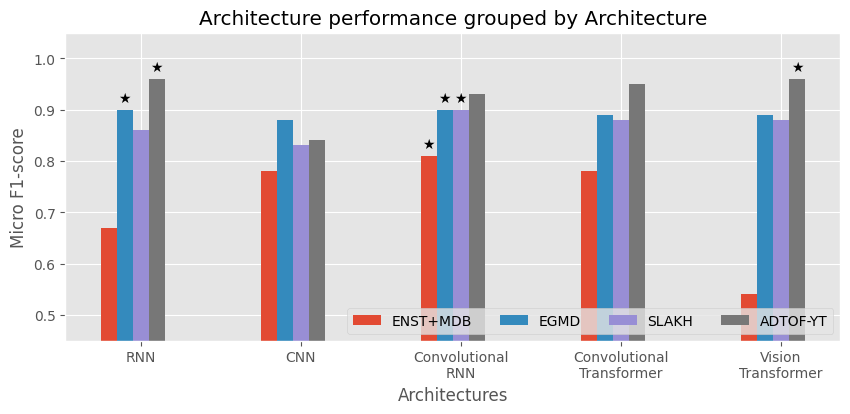
\includegraphics[scale=0.8]{figures/architectureperformancearchitecture.png}
    \caption{Test micro F1-scores per dataset, grouped by architecture. Bars marked with a ($\star$) indicate the best-performing architecture for each dataset.}
    \label{ArchitectureResultsArchitectureFigure}
\end{figure}

\begin{figure}[H]
    \centering
    \hspace*{-0.8cm}
    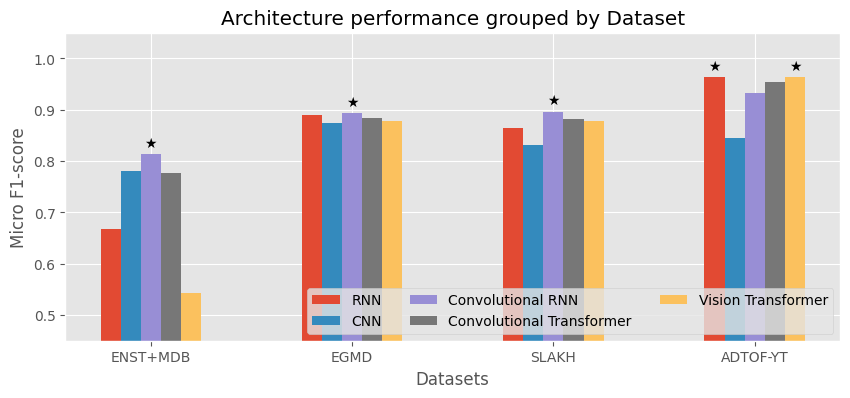
\includegraphics[scale=0.8]{figures/architectureperformancedataset.png}
    \caption{Test micro F1-scores per architecture, grouped by dataset. Bars marked with a ($\star$) indicate the best-performing architecture for each dataset.}
    \label{ArchitectureResultsDatasetFigure}
\end{figure}

\begin{figure}[H]
    \centering
    \begin{tikzpicture}
    \matrix[label=north:{\acrshort{CRNN} — ENST+MDB Sample Prediction}] {
        \node[label=west:{Target Sequence}] {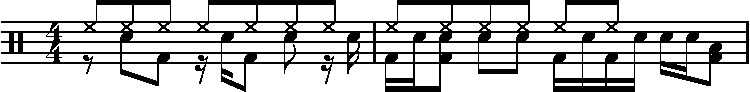
\includegraphics[scale=1.0]{lilypond/predictions/enst+mdb.cropped.pdf}}; \\
        \node[label=west:{Predicted Sequence}] {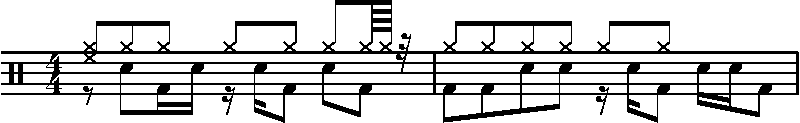
\includegraphics[scale=0.94]{lilypond/predictions/enst+mdb_prediction.cropped.pdf}}; \\};
    \end{tikzpicture}
    \caption{Prediction example from the \acrfull{CRNN} on a randomly selected sequence from the ENST+MDB test split. Both sequences were manually converted from activation function format into drum staff notation. This is a complex drum pattern, but the transcription is generally accurate. Most onsets are correctly placed and labeled, although several \acrfullpl{FP} and \acrfullpl{FN} occur.}
    \label{ArchitecturePredictionComparisonENST+MDBFigure}
\end{figure}

\begin{figure}[H]
    \centering
    \begin{tikzpicture}
    \matrix[label=north:{\acrshort{CRNN} — E-GMD Sample Prediction}] {
        \node[label=west:{Target Sequence}] {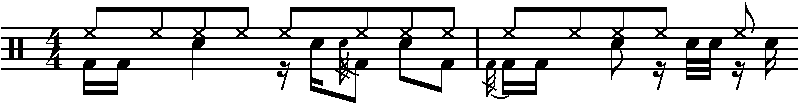
\includegraphics[scale=0.9]{lilypond/predictions/egmd.cropped.pdf}}; \\
        \node[label=west:{Predicted Sequence}] {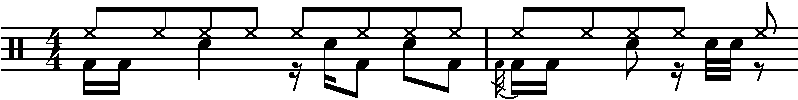
\includegraphics[scale=0.9]{lilypond/predictions/egmd_prediction.cropped.pdf}}; \\};
    \end{tikzpicture}
    \caption{Prediction example from the \acrfull{CRNN} on a randomly selected sequence from the E-GMD test split. Both sequences were manually converted from activation function format into drum staff notation. The drum pattern is moderately complex, but the model transcribed it with high accuracy. Only two \acrfullpl{FN} are present, and the prediction aligns closely with the target sequence. Note that E-GMD is a \gls{DTD} dataset without melodic accompaniment, which may make the transcription task slightly easier.}
    \label{ArchitecturePredictionComparisonEGMDFigure}
\end{figure}

\begin{figure}[H]
    \centering
    \begin{tikzpicture}
    \matrix[label=north:{\acrshort{CRNN} — Slakh Sample Prediction}] {
        \node[label=west:{Target Sequence}] {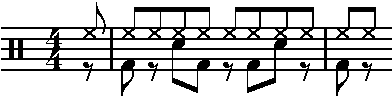
\includegraphics[scale=1.2]{lilypond/predictions/slakh.cropped.pdf}}; \\
        \node[label=west:{Predicted Sequence}] {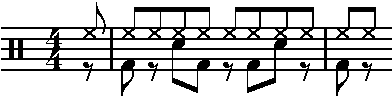
\includegraphics[scale=1.2]{lilypond/predictions/slakh_prediction.cropped.pdf}}; \\};
    \end{tikzpicture}
    \caption{Prediction example from the \acrfull{CRNN} on a randomly selected sequence from the Slakh test split. Both sequences were manually converted from activation function format into drum staff notation. The drum pattern is relatively simple, and the model produces a perfect transcription with all onsets correctly placed and labeled.}
    \label{ArchitecturePredictionComparisonSlakhFigure}
\end{figure}

\begin{figure}[H]
    \centering
    \begin{tikzpicture}
    \matrix[label=north:{\acrshort{CRNN} — ADTOF-YT Sample Prediction}] {
        \node[label=west:{Target Sequence}] {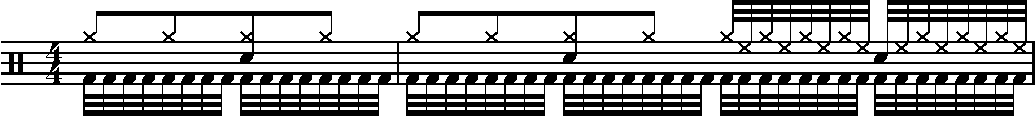
\includegraphics[scale=0.7]{lilypond/predictions/adtof_yt.cropped.pdf}}; \\
        \node[label=west:{Predicted Sequence}] {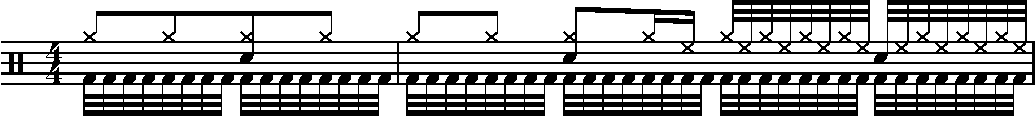
\includegraphics[scale=0.7]{lilypond/predictions/adtof_yt_prediction.cropped.pdf}}; \\};
    \end{tikzpicture}
    \caption{Prediction example from the \acrfull{CRNN} on a randomly selected sequence from the ADTOF-YT test split. Both sequences were manually converted from activation function format into drum staff notation. The pattern is dense, originating from a metal track, yet the model performs remarkably well. Only a single \acrfull{FP} is present, with all other onsets accurately transcribed.}
    \label{ArchitecturePredictionComparisonADTOF-YTFigure}
\end{figure}

\section{Discussion}

The results from the architecture study, summarized in Table~\ref{ArchitectureResultsTable} and Figures~\ref{ArchitectureResultsArchitectureFigure} and~\ref{ArchitectureResultsDatasetFigure}, indicate that there is no single architecture that consistently outperforms the others for \gls{ADT}. Instead, performance varies depending on the characteristics of each dataset and the inductive biases inherent to each architectural design.

Firstly, while multiple architectures perform well across different datasets, none emerge as universally superior. No single architecture consistently outperforms the others on all the datasets, several architectures exhibit similarly strong results depending on the dataset. 

However, the convolutional recurrent neural network demonstrates the highest micro F1-score on three of the four datasets (namely ENST+MDB, E-GMD and Slakh). It also performs strongly, but not exceptionally, on the fourth (ADTOF-YT). The consistency of its high performance across datasets with differing characteristics suggests that it is capable of handling a wide variety of \gls{ADT} tasks. This robustness appears to hold relatively independently of dataset size or complexity. 

One possible explanation for this is the architectural synergy between the convolutional and recurrent layers. The convolutional blocks provide a strong spatial feature extraction over local time–frequency patches, while the recurrent layers enable short-range temporal modeling. Together, these inductive biases may make the \gls{CRNN} especially well-suited for the challenges of \gls{ADT}.

The \acrfull{CNN} demonstrates moderate performances across all datasets. It performs adequate performance on the smallest dataset, ENST+MDB, achieving the second-highest F1-score. However, on E-GMD, Slakh and ADTOF-YT, it yields the lowest scores among the architectures, though the relative performance gap in E-GMD is minor. 

In terms of absolute F1-scores, the \gls{CNN} performs reasonably well across all datasets. Nonetheless, it consistently trails behind the other architectures, particularly on the complex and larger datasets like Slakh and ADTOF-YT. The results suggest that the \gls{CNN} is a less optimal choice for \gls{ADT}, except perhaps in scenarios with limited data or when applied on simpler tasks, such as \gls{DTD} or \acrfull{DSC}. 

More broadly, the results underscore the importance of explicitly modeling temporal dependencies in \gls{ADT}. Relying solely on the inductive biases provided by convolutional layers, such as spatially-local feature extraction, does not appear to offer sufficient flexibility to perform optimally across complex \gls{ADT} tasks.

The importance of temporal modeling is further supported by the performance of the \acrlong{RNN}. The \gls{RNN} performs surprisingly well across all datasets except the smallest, ENST+MDB. In contrast to the \gls{CNN}, it demonstrates relatively poor performance on ENST+MDB, but achieves strong results on the remaining three datasets, tying for the highest F1-score on both E-GMD and ADTOF-YT. The \gls{RNN}'s lower performance on ENST+MDB suggests that its inductive biases are weaker than those of convolutional layers, requiring more data to effectively learn the task. Notably, while it matches the \gls{CRNN} on E-GMD, it outperforms it on ADTOF-YT. This could indicate that the inductive biases introduced by convolutional layers, although powerful, may become overly dominant in certain scenarios, potentially limiting performance. Overall, the \gls{RNN} proves to be a viable architecture for \gls{ADT}, particularly when sufficient training data is available.

The convolutional transformer exhibits performance that generally falls between the \gls{RNN} and \gls{CRNN} across most datasets. It consistently achieves relatively high results, ranking just below the \gls{CRNN} on ENST+MDB, E-GMD, and Slakh, while outperforming it on ADTOF-YT. These results suggest that transformer-based models provide sufficient temporal modeling capacity to perform well on \gls{ADT} tasks. However, the findings also hint that the long-range dependencies more easily captured by attention mechanisms may be less critical than the short-range temporal aggregation offered by reccurent layers in many \gls{ADT} settings. Still, the convolutional transformer shows strong, consistent performance and can be considered a viable choice for \gls{ADT} tasks.

Finally, the \acrfull{ViT} exhibits a performance trend similar to the \gls{RNN}. On the smallest dataset, ENST+MDB, it performs notably poorly, yielding the lowest F1-score among all architectures. On E-GMD and Slakh, it achieves competitive, though not leading, results. Its performance is identical to that of the convolutional transformer. On ADTOF-YT, it performs exceptionally well, matching the highest F1-score achieved by the \gls{RNN}. 

These results reinforce earlier observations about the role of architectural inductive bias. The \gls{ViT}'s omission of convolutional layers appears to require a larger volume of high-quality data to perform well. Its underperformance on ENST+MDB further suggest that the inductive bias of attention-based architectures may be even weaker than that of recurrent layers, making them more dependent on large datasets to generalize effectively. 

This interpretation aligns with findings from existing literature, where \acrlongpl{ViT} are often shown to require an extensive amount of training data, or pretraining on large-scale dataset to achieve optimal performance~\cite{dosovitskiy2021imageworth16x16words}. Future work involving such pretraining could provide a more acurate estimate of the \gls{ViT}'s true potential in \gls{ADT}.

As shown earlier, the \acrfull{CRNN} achieves the highest F1-score on most of the datasets. While a high F1-score is a useful aggregate metric, it does not fully capture the qualitative nature of the model's predictions. To provide further insight, Figures~\ref{ArchitecturePredictionComparisonENST+MDBFigure}, \ref{ArchitecturePredictionComparisonEGMDFigure}, \ref{ArchitecturePredictionComparisonSlakhFigure}, and~\ref{ArchitecturePredictionComparisonADTOF-YTFigure} present example predictions made by the \gls{CRNN} on randomly selected sequences from the test split of each dataset. These visualizations offer a more intuitive understanding of model behavior on unseen data and further support our findings.

The ENST+MDB sample prediction is generally accurate, with many onsets correctly identified. However, it also contains several \acrfullpl{FP} and \acrfullpl{FN}. Notably, the model consistently misclassifies the \acrfull{HH} onsets as \acrfull{CC+RC}, and missed occasional fast, closely spaced \acrfull{SD} onsets. Given the small size of ENST+MDB and the complexity of this particular sequence, the prediction remains reasonable overall.

In contrast, the three other sample predictions are remarkably accurate. Two are nearly flawless, while the third is entirely correct. Across these three examples, only a single \acrshort{FP} and two \acrshortpl{FN} are observed. These samples also span a range of difficulty: the Slakh transcription is relatively simple, E-GMD is moderately complex, and ADTOF-YT is highly dense with a moderate rhythmic intricacy. The \gls{CRNN}'s ability to handle this spectrum of complexity while maintaining a high prediction accuracy, is notable.

Although each model was trained and evaluated within its own dataset domain, these examples provide helpful intuition into how the \gls{CRNN}'s high F1-scores translate to real-world transcription performance.

It is important to acknowledge the potential sources of variability that may influence the results of this study. Factors such as random weight initialization, stochastic hyperparameter sampling, numerical precision limits, and dataset-specific variability (e.g., differences in splits or noise artifacts) can all impact model performance. However, several design choices help mitigate these effects. Training a substantial number of models per experiment, using batch sizes that average out gradient noise, and relying on predefined, independently curated train, validation and test splits all contribute to stabilizing the evaluation. These measures increase the likelihood that the observed performance differences primarily reflect the influence of architecture choice, rather than random variation.

Taking this into account, my results strongly suggest that the \acrfull{CRNN} is the most effective architecture for \gls{ADT} across the datasets studied. It achieved the highest micro F1-scores on most benchmarks and produced accurate transcriptions in qualitative visualizations. That said, further research should continue to explore the scalability of both \acrfullpl{RNN} and the \acrfull{ViT}, particularly how they perform on larger datasets and, for the latter, in conjunction with pretraining schemes. Such investigations may offer deeper insight into these models' full potential for \gls{ADT} tasks.